% Options for packages loaded elsewhere
\PassOptionsToPackage{unicode}{hyperref}
\PassOptionsToPackage{hyphens}{url}
%
\documentclass[
  10pt,
]{article}
\usepackage{amsmath,amssymb}
\usepackage{iftex}
\ifPDFTeX
  \usepackage[T1]{fontenc}
  \usepackage[utf8]{inputenc}
  \usepackage{textcomp} % provide euro and other symbols
\else % if luatex or xetex
  \usepackage{unicode-math} % this also loads fontspec
  \defaultfontfeatures{Scale=MatchLowercase}
  \defaultfontfeatures[\rmfamily]{Ligatures=TeX,Scale=1}
\fi
\usepackage{lmodern}
\ifPDFTeX\else
  % xetex/luatex font selection
    \setmainfont[]{Times New Roman}
\fi
% Use upquote if available, for straight quotes in verbatim environments
\IfFileExists{upquote.sty}{\usepackage{upquote}}{}
\IfFileExists{microtype.sty}{% use microtype if available
  \usepackage[]{microtype}
  \UseMicrotypeSet[protrusion]{basicmath} % disable protrusion for tt fonts
}{}
\makeatletter
\@ifundefined{KOMAClassName}{% if non-KOMA class
  \IfFileExists{parskip.sty}{%
    \usepackage{parskip}
  }{% else
    \setlength{\parindent}{0pt}
    \setlength{\parskip}{6pt plus 2pt minus 1pt}}
}{% if KOMA class
  \KOMAoptions{parskip=half}}
\makeatother
\usepackage{xcolor}
\usepackage[left=2cm, right=2cm,top=2cm, bottom=2cm]{geometry}
\usepackage{graphicx}
\makeatletter
\def\maxwidth{\ifdim\Gin@nat@width>\linewidth\linewidth\else\Gin@nat@width\fi}
\def\maxheight{\ifdim\Gin@nat@height>\textheight\textheight\else\Gin@nat@height\fi}
\makeatother
% Scale images if necessary, so that they will not overflow the page
% margins by default, and it is still possible to overwrite the defaults
% using explicit options in \includegraphics[width, height, ...]{}
\setkeys{Gin}{width=\maxwidth,height=\maxheight,keepaspectratio}
% Set default figure placement to htbp
\makeatletter
\def\fps@figure{htbp}
\makeatother
\setlength{\emergencystretch}{3em} % prevent overfull lines
\providecommand{\tightlist}{%
  \setlength{\itemsep}{0pt}\setlength{\parskip}{0pt}}
\setcounter{secnumdepth}{-\maxdimen} % remove section numbering
\usepackage{booktabs}
\usepackage{longtable}
\usepackage{array}
\usepackage{multirow}
\usepackage{wrapfig}
\usepackage{float}
\usepackage{colortbl}
\usepackage{pdflscape}
\usepackage{tabu}
\usepackage{threeparttable}
\usepackage{threeparttablex}
\usepackage[normalem]{ulem}
\usepackage{makecell}
\usepackage{xcolor}
\ifLuaTeX
  \usepackage{selnolig}  % disable illegal ligatures
\fi
\usepackage{bookmark}
\IfFileExists{xurl.sty}{\usepackage{xurl}}{} % add URL line breaks if available
\urlstyle{same}
\hypersetup{
  pdftitle={Estimation And Prediction Of Patient Length Of Stay},
  pdfauthor={Ya Wang, Yu Qing, Suyuan Wang, Yile Zhu},
  hidelinks,
  pdfcreator={LaTeX via pandoc}}

\title{Estimation And Prediction Of Patient Length Of Stay}
\usepackage{etoolbox}
\makeatletter
\providecommand{\subtitle}[1]{% add subtitle to \maketitle
  \apptocmd{\@title}{\par {\large #1 \par}}{}{}
}
\makeatother
\subtitle{\url{https://github.com/ZYLwayne/Biostat625-Final-Project}}
\author{Ya Wang, Yu Qing, Suyuan Wang, Yile Zhu}
\date{}

\begin{document}
\maketitle

\section{Abstract}\label{abstract}

Increasing healthcare costs and the availability of large amounts of
healthcare data have led to a search for ways to improve the efficiency
of healthcare. Length of stay (LOS) and its impact have significant
economic and human implications, and therefore the prediction of this
key parameter has been the subject of research in recent years. The aim
of this paper is to explore the key factors affecting the length of stay
(LOS) of patients and to predict the length of stay through a variety of
machine learning models. The study uses a dataset containing 28,109
records covering demographic characteristics, admission type and cost
information. We found that patients with longer lengths of stay were
concentrated in the 70+ age group, male patients, black or African
American, and hospital service areas in New York City and the Southland.
In addition, trauma admissions had significantly longer lengths of stay
than other admission types. Whereas there was a significant linear
relationship between total charges and total costs (R² = 0.8046, p
\textless{} 2e-16), costs emerged as a significant predictor of length
of stay. Notably this study compared the performance of three models:
linear regression, CART (Classification and Regression Trees) and Random
Forest and further assessed their stability through cross-validation
(CV). The results showed that the random forest model achieved the
lowest RMSE(8.83) among all models, demonstrating its superiority in
capturing complex nonlinear relationships and feature interactions. In
addition, the findings provide data support and decision-making basis
for hospitals in cost management, resource allocation, and high-risk
patient identification.

\section{1. Introduction}\label{introduction}

With rising healthcare expenses and increased access to big data in
healthcare, how to effectively improve the efficiency of healthcare
systems has become a critical issue that must be addressed. Length of
Stay (LOS) is an important metric for assessing hospital operational
efficiency and healthcare service quality, as it is not only closely
related to resource allocation but also has a significant impact on
patient recovery and hospital cost management{[}1{]}. As a result, in
recent years, precise estimation and prediction of length of stay has
emerged as a key area of academic research and practice{[}2{]}.

The goal of this project is to employ a data-driven strategy to
investigate and predict the important characteristics that determine the
length of a patient's hospital stay using various machine learning
models. We use a huge dataset of 28,109 records published by the New
York State Department of Health, which includes information about
patient demographics, type of admission, and cost. During the data
modeling step, three predictive models were built: Linear Regression,
Classification and Regression Tree (CART), and Random Forest, and the
models' stability was evaluated using Cross-Validation{[}3{]}.

The paper is organized as follows:

The second section will introduce the dataset and the data preprocessing
process, including missing value processing, feature engineering and
data segmentation.

The third section compares and analyses the model results to reveal the
importance of key variables.

The fourth part summarises the research results and proposes suggestions
for improvement and future research directions.

This study will give hospital administrators with an effective data
analysis tool to help enhance the precision of healthcare resource
allocation, hence improving the patient's hospitalization experience and
lowering total healthcare expenses{[}4{]}.

\section{2. Methodology}\label{methodology}

\subsection{2.1 Data Processing}\label{data-processing}

The dataset used in this study was derived from the New York State
region's hospital management system and recorded patient hospitalisation
data from mid-2022. The dataset contains 28,109 records and 23
variables, mainly including the target variable: Length.of.Stay
(continuous variable indicating the number of days the patient was
hospitalised.) and characteristic variables including numeric variables
(e.g.~Discharge.Year, APR.DRG.Code, APR.Severity.of.Illness.Code,
Total.Charges, Total.) and categorical variables:
(e.g.~Hospital.Service.Area, Age.Group, Gender, Race, Ethnicity,
Type.of.Admission, etc.).

\subsubsection{2.1.1 Data Cleaning}\label{data-cleaning}

\begin{enumerate}
\def\labelenumi{(\arabic{enumi})}
\item
  Variables (Payment.Typology.3) and (Payment.Typology.2) were excluded
  due to high missing values (83\% and 41\%, respectively).
\item
  For variables with minimal missing values (e.g., Ethnicity, Gender,
  Hospital.Service.Area), missing data were filled using mode
  imputation.
\item
  Columns with a single unique value, such as CCSR.Diagnosis.Code and
  CCSR.Diagnosis.Description, were removed to eliminate redundancy.
\end{enumerate}

\subsubsection{2.1.2 Data Transformation and One-Hot
Encoding}\label{data-transformation-and-one-hot-encoding}

\begin{enumerate}
\def\labelenumi{(\arabic{enumi})}
\item
  Logarithmic Transformation: Continuous numerical variables
  (Total.Charges, Total.Costs, Length.of.Stay) were log-transformed to
  normalize skewed distributions and reduce the impact of outliers.
\item
  Categorical variables were transformed into binary vectors using
  one-hot encoding while removing the first dummy to avoid
  multicollinearity.
\end{enumerate}

\subsection{2.2 Data Segmentation}\label{data-segmentation}

70-30 Train-Test Split: The dataset will be split into 70\% for training
and 30\% for testing, ensuring model generalization and reducing
overfitting.

\subsection{2.3 Model Development}\label{model-development}

Linear regression is a classical statistical method used to study the
linear relationship between a dependent variable (target variable) and
one or more independent variables (predictor variables). For multiple
linear regression, the model equation is: \[
Y = \beta_0 + \beta_1X_1 + \beta_2X_2 + \cdots + \beta_nX_n + \varepsilon
\]

The CART model is a classification and regression method based on a tree
structure for dealing with nonlinear relationships and variable
interactions.

Random forest is an integrated learning method that consists of multiple
decision trees that are integrated to improve the accuracy and stability
of the model. It has high prediction accuracy, high generalization
ability and can handle non-linear relationships and interactions between
features.

\subsection{2.4 Model performance
evaluation}\label{model-performance-evaluation}

In order to comprehensively compare the performance of different models,
this study adopts Root Mean Square Error (RMSE) as the main assessment
metric. And the cross validation method is added to test the models, and
finally the comparison of the computational model performance is based
on the results of No-Cross Validation (No-CV) and With-CV{[}5{]}.

In this study, the root mean square error (RMSE) is calculated as:
\(RMSE = \sqrt{\frac{\sum_{i=1}^n (y_i - \hat{y}_i)^2}{n}}\)

\section{3. Result}\label{result}

\subsection{3.1 Distribution of Demographics in terms of Length of
Stay}\label{distribution-of-demographics-in-terms-of-length-of-stay}

By looking at the distribution of demographic data under Length of Stay,
it can be seen that Hospital.Service.Area, Age.Group, Gender, and Race
are all significantly different (p value \textless{} 0.05) from the
distribution of Length of Stay under Group, except for Ethnicity.

\begin{verbatim}
(1) it can be seen that patients in New York City, Southern Tier have longer Length of Stay relative to other regions.
(2) The older the patient, the longer the Length of Stay.
(3) Male patients have a longer Length of Stay than female patients.
(4) Length of Stay is longer for patients of Black/African American race.
\end{verbatim}

\begin{figure}
\centering
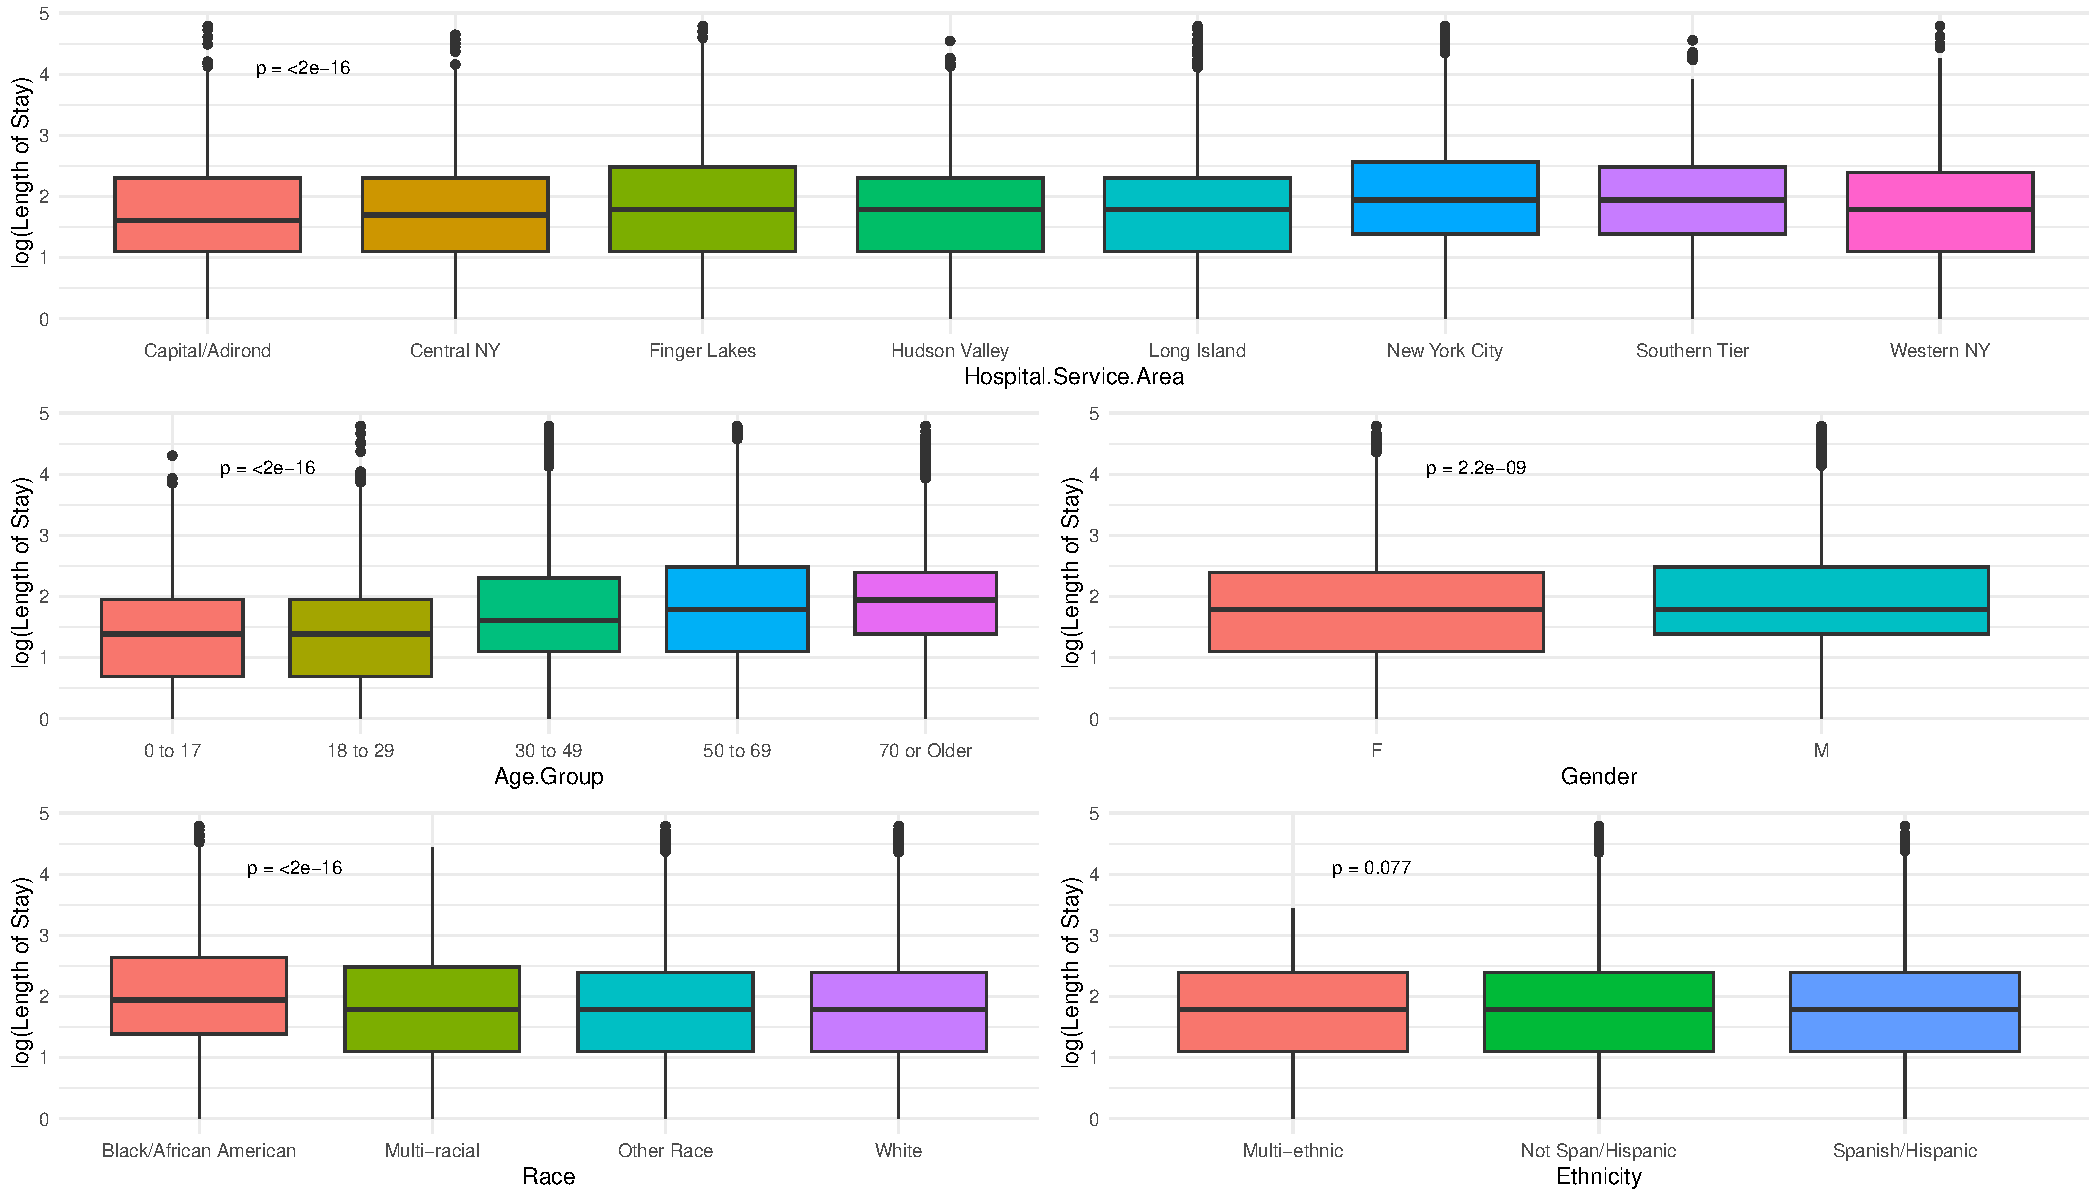
\includegraphics{Biostat625_Final-Projet_files/figure-latex/unnamed-chunk-1-1.pdf}
\caption{Boxplot for Distribution of Demographics in terms of Length of
Stay}
\end{figure}

\subsection{3.2 Distribution of Admission Information in terms of Length
of
Stay}\label{distribution-of-admission-information-in-terms-of-length-of-stay}

There was a statistically significant difference between
Type.of.Admission, Emergency Department Indicator and Length of Stay,
all with p-values less than 0.05.

\begin{enumerate}
\def\labelenumi{(\arabic{enumi})}
\item
  Trauma patients have a higher median length of stay than other types
  of hospitalization. Trauma patients are usually admitted to the
  hospital as a result of an accident or severe trauma, and these
  patients tend to have more complex conditions that may require
  multiple tests, treatments, and surgeries. These patients may be
  accompanied by multiple comorbidities, leading to a longer course of
  treatment, which in turn increases the number of hospital days.
\item
  Non-emergency hospitalized patients may require multiple treatments or
  post-surgical recoveries, resulting in additional days of
  hospitalization. Emergency patients, despite being more severely ill,
  may have shorter hospital stays due to better emergency care and
  treatment standards. Second, non-emergency patients may face stricter
  discharge criteria, and hospitals may take longer to assure patient
  recovery and stability, influencing the median number of hospital
  days.
\end{enumerate}

\begin{figure}
\centering
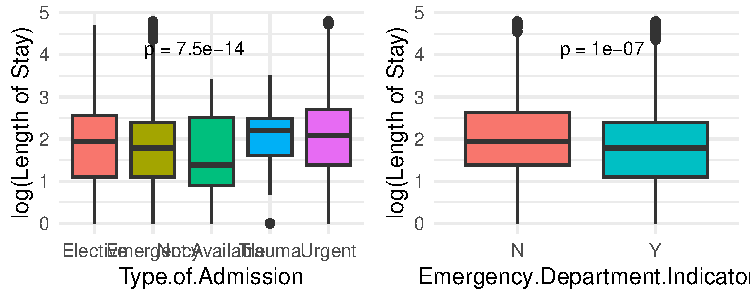
\includegraphics{Biostat625_Final-Projet_files/figure-latex/unnamed-chunk-2-1.pdf}
\caption{Boxplot for Distribution of Admission Information in terms of
Length of Stay}
\end{figure}

\subsection{3.3 Linear relationship between Charges and
Costs}\label{linear-relationship-between-charges-and-costs}

By building a linear regression model after logarithmic transformation
of the relationship between Total Charges for hospitalization (Total
Charges) and Total Costs, we observed that the two showed a significant
linear relationship, and each parameter in the model had a very high
level of significance (p \textless{} 2e-16), which demonstrated the
validity and reliability of the model; the value of the multiple R² is
0.8046, indicating that about 80.46\% of the total cost variation can be
explained by the total cost variation. The skewness values of Total
Charges and Total Costs (0.242 and 0.376, respectively) indicate that
the distribution is close to normal and the data distribution is more
concentrated.

\begin{enumerate}
\def\labelenumi{(\arabic{enumi})}
\item
  Cost reasonableness: by building this linear regression model,
  hospitals are able to predict hospitalization costs more accurately
  and set reasonable fees based on costs. This helps hospitals to be
  more transparent and fair in setting fees and avoid unnecessary and
  indiscriminate charging.
\item
  Cost control: Hospital management can use this model to evaluate the
  costs and corresponding charges for different medical services to
  ensure that the fees match the actual costs. This not only helps to
  improve the financial transparency of the hospital, but also helps to
  enhance patients' trust in hospital charges.
\end{enumerate}

\begin{figure}
\centering
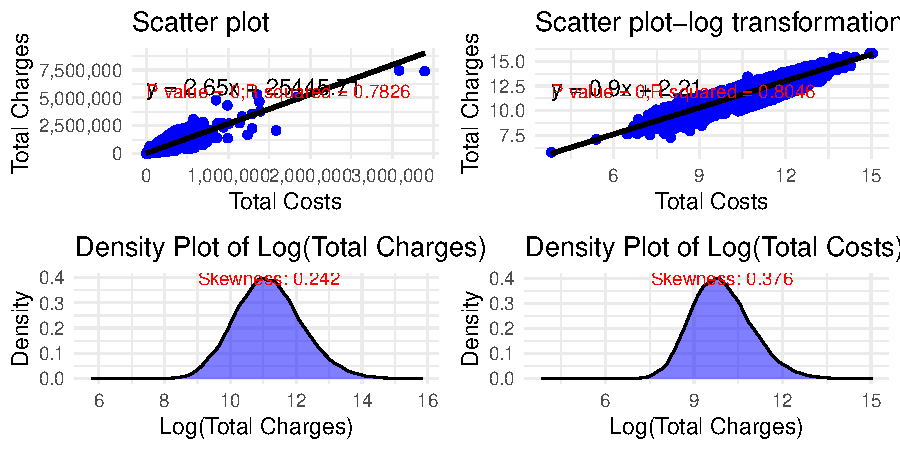
\includegraphics{Biostat625_Final-Projet_files/figure-latex/unnamed-chunk-3-1.pdf}
\caption{Linear relationship between Charges and Costs}
\end{figure}

\subsection{3.4 Model evaluation and
comparison}\label{model-evaluation-and-comparison}

Comparing the performance of the three models together, the Random
Forest model performed the best:

The RMSE of Random Forest (8.83 without CV, 0.3968 with CV), shows
strong nonlinear modelling and generalisation capabilities. Compared to
linear regression and CART, Random Forest is more advantageous in
dealing with complex data features, and is especially suitable for
high-dimensional datasets containing nonlinear relationships and
interactions.

\begin{table}
\centering
\caption{\label{tab:unnamed-chunk-6}RMSE for the three models}
\centering
\fontsize{7}{9}\selectfont
\begin{tabular}[t]{lrr}
\toprule
Model & RMSE\_No\_CV & RMSE\_With\_CV\\
\midrule
\cellcolor{gray!10}{Linear Regression} & \cellcolor{gray!10}{13.047861} & \cellcolor{gray!10}{0.4074009}\\
CART & 9.639912 & 0.5997748\\
\cellcolor{gray!10}{Random Forest} & \cellcolor{gray!10}{8.833774} & \cellcolor{gray!10}{0.3968267}\\
\bottomrule
\end{tabular}
\end{table}

\section{4. Conclusion}\label{conclusion}

In-depth analyses of length of stay data revealed that length of stay
was significantly longer for older patients (70 years and older), male
patients, black or African American patients, and patients from the New
York City and Southern Tier Hospital service areas. Furthermore, trauma
admissions were much longer than other admission types, and hospital
expenses (Total.expenses and Total.Charges) were strongly positively
connected with hospital length of stay, with linear regression analyses
revealing a significant positive relationship. In the model performance
comparison, although linear regression can effectively capture linear
relationships, it is difficult to deal with the nonlinear features in
the data (RMSE = 13.05); the CART model captures some of the nonlinear
relationships through the tree structure, which improves the performance
(RMSE = 9.64); and the Random Forest model performs the best (RMSE =
8.83), which can effectively deal with the nonlinear relationship and
the interaction between variables interactions, with the highest
prediction accuracy and generalisation ability.

Research Recommendations and Improvements: more accurate filling methods
(e.g., KNN filling or machine learning prediction) can be explored for
the handling of missing data. The introduction of interaction terms and
more advanced feature engineering can also be considered to further
improve model performance.

Overall, this work provides an important decision-making foundation for
optimizing hospital resource allocation, controlling costs, and managing
high-risk patients, and it can be coupled with other machine learning
models in the future to improve prediction effect and model
interpretability.

\section{References}\label{references}

\begin{enumerate}
\def\labelenumi{\arabic{enumi}.}
\tightlist
\item
  Robinson G H, Davis L E, Leifer R P. Prediction of hospital length of
  stay{[}J{]}. Health services research, 1966, 1(3): 287.
\item
  Clarke A, Rosen R. Length of stay: how short should hospital care
  be?{[}J{]}. The European Journal of Public Health, 2001, 11(2):
  166-170.
\item
  Lequertier, Vincent, et al.~``Hospital length of stay prediction
  methods: a systematic review.'' Medical care 59.10 (2021): 929-938.
\item
  Robinson G H, Davis L E, Leifer R P. Prediction of hospital length of
  stay{[}J{]}. Health services research, 1966, 1(3): 287.
\item
  Verburg, Ilona WM, et al.~``Comparison of regression methods for
  modeling intensive care length of stay.'' PloS one 9.10 (2014):
  e109684.
\end{enumerate}

\section{Contribution}\label{contribution}

Ya Wang: Contributions include building random forest models, data
processing and cleaning, and report writing. Suyuan Wang: Contributions
include building linear regression models, data analysis and processing,
and report writing. Yu Qing: Contributions include building cart models,
data analysis and processing, and report writing. Yile Zhu:
Contributions have identified datasets and code frameworks, model
visualisation and comparative analysis of results, integrated reports

\end{document}
